%%%%%%%%%%%%%%%%%%%%%%%%%%%%%%%%%%%%%%%%%%%%%%%%%%%%%%%%%%%%%%%%%%%%%%%%%%%%%%%%%%%%%%%%%%%%%
\subsection{Overview}
In this chapter we are going to illustrate the approaches that we have implemented, in particular we will discuss about MudaBlue,Clan, RepoPal and CrossSim. As explained before, the purpose is to provide a baseline to evaluate CrossSim, so it's mandatory to have a precise idea of what these approaches are and how does they work. Concerning MudaBlue and Clan, we will discuss about their rationale, showing also their original results, then we will show how we reimplemented such approaches from an high-level point of view.


\subsection{MUDABlue}\label{sec:mudablue}

The first procedure analysed was MUDABlue, unfortunately none implentation was available on the web, so i reimplemented it from scratch. The MUDABlue method is an automatc categorizaton method of a large collecton of software systems. MUDABlue method does not only categorize sooware systems but also determines categories from the software systems collection automatigcally. MUDABlue has three major aspects: 1) it relies on no other information than the source code, 2) it determines category sets automatically, and 3) it allows a software system to be a member of multiple categories. Since we were interested only in the evaluation of the similarity we discarded the phases related to clusterization and categorization.

The MUDABlue approach can be briefly summarized in 7 steps, as the following image depicts:

\begin{figure}[H]
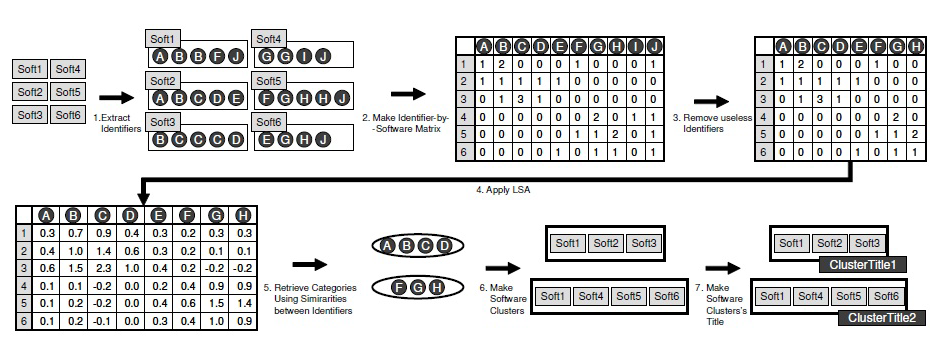
\includegraphics[width=15cm,height=20cm,keepaspectratio]{images/Mudablue1.png}
\centering
\caption{MUDABlue phases.}
\end{figure}

\subsubsection{Exctract Identifiers}
With identifier we are talking about relevant strings that can allow to characterize a document. In this phase each repository is scanned in order to find the target files, and for each of them the identifiers are exctracted, avoiding adding useless items such as comments. The dataset was a 41C projects gathered from SourceForge.

\subsubsection{Create identifier-by-software matrix}
As stated before, the main item to work with is the term-document matrix, in this case we count how many times each term appears in each file for all the projects. The result is matrix \textbf{m x n} with m terms and n projects.

\subsubsection{Remove useless identifiers}
From the matrix we remove all the useless terms, that is all the terms that apperas in just one repository, considered a specific terms, and all the terms that appears in more than 50\% of the repositories, considered as general terms.

\subsubsection{Apply the LSA}
Once the matrix is ready con be worked, the \emph{SVD} procedure is applied and then the LSI. As explained before [NOTE] the \emph{SVD} procedure decompose the original matrix in 3 other matrices. When we multiply back these matrices we use a rank reducted version of the S matrix in order to generete the final one. The authors didn't provide us any details about their final rank value, so we tested many values and eventually selected one.

\subsubsection{Apply the Cosine Similarity}
By using the cosine similarity method, we compare each repository vector with all the others and eventually getting an \textbf{n x n} matrix, in which is expressed the similarity of all the repository couple, with a value \emph{[0.0-1.0]}. Thereafter, the cluster analysis is applied using calculated similarities. 

\subsubsection{Categorization}
Make software clusters from identifier clusters. From each identifier clusters, the software systems that contain one or more identifiers in the cluster are retrieved. The last step is to make software clusters’ titles. This can be done by summing all identifier-vectors comprised in the identifier cluster and then consider the ten identifiers that got the highest value in the summation vector.

\subsubsection{Results}
The experimentation was conducted on a corpus of $41$ \emph{C} projects, taken form SourceForge belonging to $5$ categories.
Developers used \emph{precision} and \emph{recall} as criteria, defined as follows:

\begin{equation}
Precision = \frac{\sum_{s\in S}\text{precision}_{soft}\text{(S)}}  {\mid S \mid}
\end{equation}

\begin{equation}
Recall = \frac{\sum_{s\in S}\text{recall}_{soft}\text{(S)}}  {\mid S \mid}
\end{equation}

\begin{equation}
Precision_{soft}\text{(s)} = \frac{\mid C_\text{MudaBlue}\text{(s)} \cap C_\text{Ideal}\text{(s)} \mid}  {\mid C_\text{MudaBlue}\text{(S)} \mid}
\end{equation}

\begin{equation}
Recall_{soft}\text{(s)} = \frac{\mid C_\text{MudaBlue}\text{(s)} \cap C_\text{Ideal}\text{(s)} \mid}  {\mid C_\text{Ideal}\text{(s)} \mid}
\end{equation}

where $C_\text{MudaBlue}\text{(s)}$ is a set of categories containing software s, generated by MUDABlue, $C_\text{Ideal}\text{(s)}$ is a set of categories containing software \emph{s}, determined manually by the experimenters. In both of the criteria, the larger value,
the better result.

\clearpage


%%%%%%%%%%%%%%%%%%%%%%%%%%%%%%%%%%%%%%%%%%%%%%%%%%%%%%%%%%%%%%%%%%%%%%%%%%%%%%%%%%%%%%%%%%%%%

\subsection{CLAN:  Closely reLated ApplicatioNs}\label{sec:clan}

\textit{CLAN} \cite{McMillan:2012:DSS:2337223.2337267} is an approach for automatically detecting similar Java applications by exploiting the semantic layers corresponding to packages class hierarchies. \textit{CLAN} works based on the document framework for computing similarity, semantic anchors, e.g. those that define the documents' semantic features. Semantic anchors and dependencies help obtain a more precise value for similarity computation between documents. The assumption is that if two applications have API calls implementing requirements described by the same abstraction, then the two applications are more similar than those that do not have common API calls. The approach uses API calls as semantic anchors to compute application similarity since API calls contain precisely defined semantics. The similarity between applications is computed by matching the semantics already expressed in the API calls.

The process consist of 12 steps here graphically reported.

\begin{figure}[H]
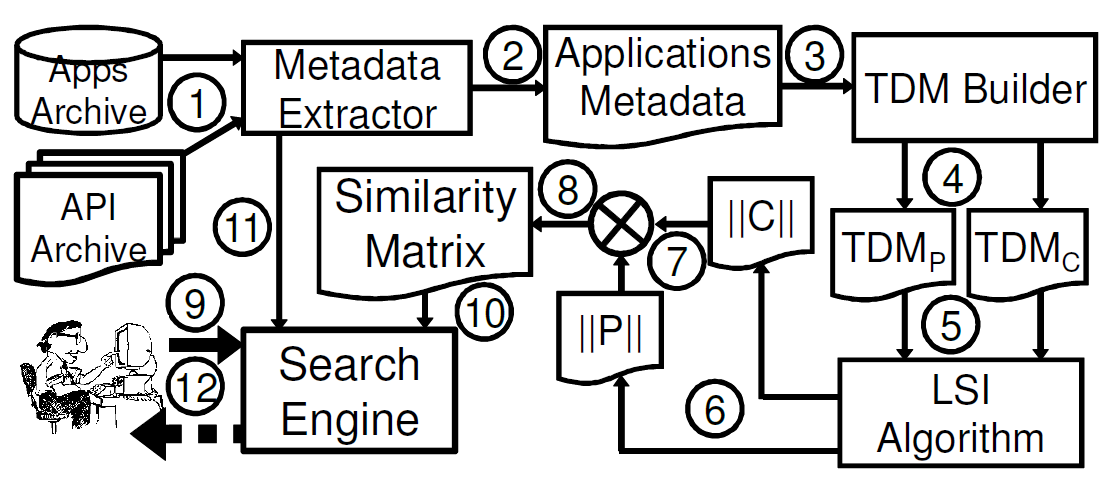
\includegraphics[width=15cm,height=20cm,keepaspectratio]{images/Clan.png}
\centering
\caption{CLAN phases.}
\end{figure}

\subsubsection{Terms Extraction}
Steps from 1 to 3 can be merged together since are related to extraction of terms from the repositories.
As stated before, an important concept is that terms extracted are only API calls, this means that all other things present in a piece of code are discarded, for example all the variables or the function declaration and invocation. Furthermore these API calls belong only to the JDK, in such a way also the calls to any other external library are discarded. This idea is also applied in the extraction of the import declaration, focus only on the JDK packages import.
The result of this process will be an ordered set of data, representing the occurrencies of any Package;Class for all the projects.

\subsubsection{TDMs Creation}
Once the dataset as been created, is reorganized in TDMs. Here two different matrices are created, one for the Classes and one for the Packages. Class-level and package-level similarities are different since applications are often more similar on the package level than on the class level because there are fewer packages than classes in the JDK. Therefore, there is the higher probability that two applications may have API calls that are located in the same package but not in the same class.

\subsubsection{LSI Procedure}
The paper refers to LSI procedure, Latent Semantic Indexing[dumais2], but the term are synonym, so from here on, we will refer as Latent Semantic Analysis LSA.

\subsubsection{Apply the Cosine Similarity}
As for Mudablue, we will apply the cosine similarity to the matrix got from the LSA procedure.

\subsubsection{Sum of the matrices}
The 2 matrices are summed, but before are multplied by a certain value. Since the values for the entries in the 2 matrices are between 0.0 and 1.0 a simple sum could result in a value over 1.0, by this multiplication these values are reducted in order to be summed togheter but still maintaining the logical meaning. The authors chosen 0.5, also we, since is a good value to equal distribute the weight of the packages and method calls.The sum of this value is 1.0, and can span from 0.1 to 0.9 for each matrix, is clear that more is high on a matrix, more is important the values that we are considering from such matrix.

\subsubsection{Final similarity matrix}
Once the matrix is ready, the system will use it to answer the query of users, from such  matrix the system will retrieve the common projects ordered by rank.

\subsubsection{Results}
The developers used a corpus of $8310$ projects from SourceForge, for a total of $114146$ API calls. The evaluation method was similar to our, a user study with a group of 33 student of University of Illinois at Chicago with at least 6 months of java experience. Their main task was to examine the retrieved applications and to determine if they are relevant to the tasks and the source application. Each participant accomplished this step individually, assigning a confidence level, C, to the examined applications using a four-level Likert scale.

\begin{figure}[H]
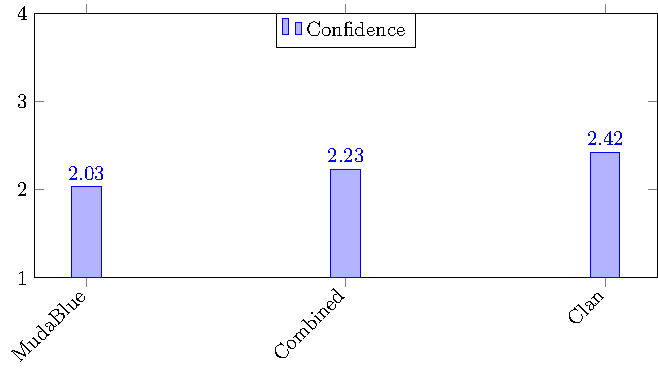
\includegraphics[width=10cm,height=15cm,keepaspectratio]{images/ConfidenceClan.pdf}
\centering
\caption{Confidence Comparison Original Clan}
\label{fig:ConfidenceClan}
\end{figure}

\begin{figure}[H]
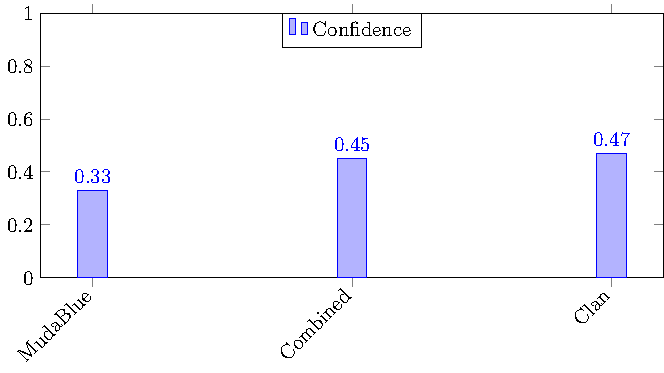
\includegraphics[width=10cm,height=15cm,keepaspectratio]{images/PrecisionClan.pdf}
\centering
\caption{Precision Comparison Original Clan}
\label{fig:PrecisionClan}
\end{figure}

Figure \ref{fig:ConfidenceClan} and figure \ref{fig:PrecisionClan} reports the mean of the results they got from the students. As you can see the Clan approach performs better than MudaBlue. Since Similarity Matrices of MUDABlue and CLAN have the same dimensions, it is possible to construct a combined matrix whose values are the average of the values of the MUDABlue and CLAN matrix elements at the
corresponding position. [nota e chiedere]
\clearpage


%%%%%%%%%%%%%%%%%%%%%%%%%%%%%%%%%%%%%%%%%%%%%%%%%%%%%%%%%%%%%%%%%%%%%%%%%%%%%%%%%%%%%%%%%%5  

\subsection{RepoPal: Exploiting Metadata to Detect Similar GitHub Repositories}\label{sec:repopal}

In contrast to many previous studies that are generally based on source code \cite{10.1109/APSEC.2004.69},\cite{Liu:2006:GDS:1150402.1150522},\cite{McMillan:2012:DSS:2337223.2337267}, \textit{RepoPal}  \cite{10.1109/SANER.2017.7884605} is a high-level similarity metric and takes only repositories metadata as its input. With this approach, two GitHub repositories are considered to be similar if:

\begin{itemize}
	\item[i)] They contain similar readme files;
	\item[ii)] They are starred by users of similar interests;
	\item[iii)] They are starred together by the same users within a short period of time. 
\end{itemize}

Thus, the similarities between GitHub repositories are computed by using three inputs: readme file, stars and the time gap that a user stars two repositories. Considering two repositories $ r_{i} $ and $ r_{j} $, the following notations are defined: 

\begin{itemize}
	\item $ f_{i} $ and $ f_{j} $ are the readme files with $ t $ being the set of terms in the files; 
	\item $ U(r_{i}) $ and $ U(r_{j}) $ are the set of users who starred $ r_{i} $ and $ r_{j} $, respectively; 
	\item $ R(u_{k}) $ is the set of repositories that user $ u_{k} $ already starred.  
\end{itemize}

There are three similarity indices as follows:

\paragraph{Readme-based similarity} 

The similarity between two readme files is calculated as the cosine similarity between their feature vectors $\vec{f_{i}}$ and $\vec{f_{j}}$: 

\begin{equation}
sim_{f}(r_{i},r_{j})=CosineSim(\vec{f_{i}},\vec{f_{j}})
\end{equation}
\clearpage

%%%%%%%%%%%%%%%%%%%%%%%%%%%%%%%%%%%%%%%%%%%%%%%%%%%%%%%%%%%%%%%%%%%%%%%%%%%%%%%%%%
\subsection{CrossSim}

Since the purpose of this thesis is to provide implementation and data to validate CrossSim approach, is useful to explain in detail it.
So this section we are going to present CROSSSIM (Cross Project Relationships for Computing Open Source Software Similarity), an approach that makes use of graphs for representing different kinds of relationships in the OSS ecosystem. In particular, with the adoption of the graph representation, we are able to transform the relationships among non-human artifacts, e.g. API utilizations,
source code, interactions, and humans, e.g. developers into a mathematically computable format, i.e. one that facilitates various types of computation techniques.
 
\begin{figure}[H]
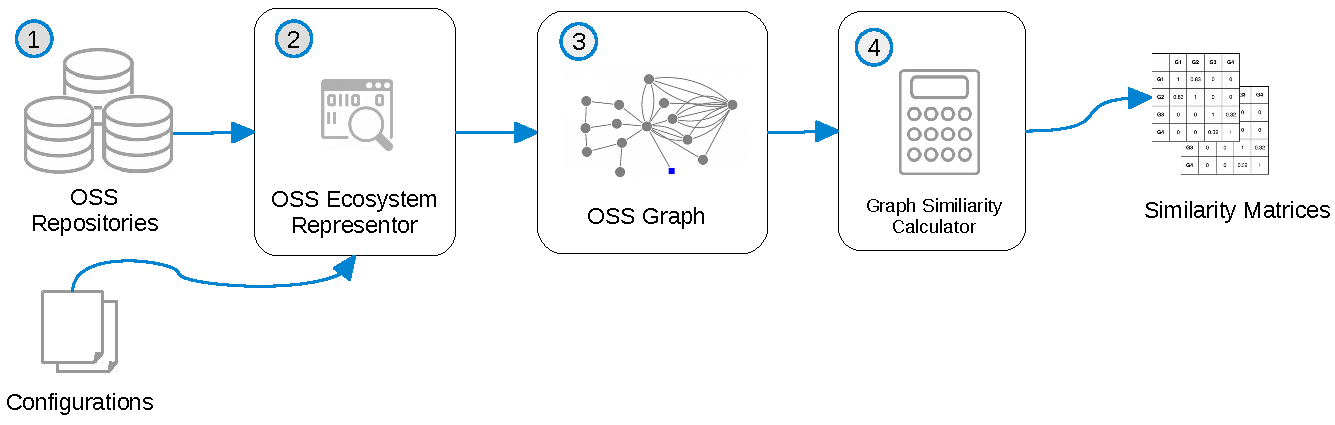
\includegraphics[width=15cm,height=20cm,keepaspectratio]{images/CrossSim.pdf}
\caption{CrossSim Structure}
\label{fig:CrossSim}
\end{figure}

The architecture of CrossSim is depicted in Fig. \ref{fig:CrossSim}: the rectangles represent artifacts, whereas the ovals represent activities that are automatically performed by the developed CrossSim tooling. In particular, the approach imports project data from existing OSS repositories and represents them into a graph-based representation by means of the \emph{OSS Ecosystem Representation} module. Depending on the considered repository (and thus to the information that is available for each project) the graph structure to be generated has to be properly configured. For instance in case of GitHub, specific configurations have to be specified in order to enable the representation in the target graphs of the stars assigned to each project. Such a configuration is ``forge'' specific and specified once, e.g., SourceForge does not provide the star based system available in GitHub. 
%
The \emph{Graph similarity} module implements the similarity algorithm that is applied on the source graph-based representation of the input ecosystems generates matrices representing the similarity value for each pair of input projects. 

\subsubsection{Graph-based Representation of OSS Ecosystems}
We consider the community of developers together with OSS projects, libraries and their mutual interactions as an \emph{ecosystem}. In this system, either humans or non-human factors have mutual dependency and implication on the others. There, several connections and interactions prevail, such as developers commit to repositories, users star repositories, or projects contain source code files, just to name a few. We propose a solution that makes use of graphs for representing relationships in OSS ecosystems. Specifically, the graph model has been chosen since it allows for flexible data integration and facilitates numerous similarity metrics and clustering techniques \cite{Blondel:2004:MSG:1035533.1035557},\cite{Lu2007},\cite{Schaeffer:2007:SGC:2296006.2296057}. All the playing actors and their communications are transformed into a directed graph. Humans and non-human artifacts are represented as nodes and there is a directed edge between a pair of nodes if they interact with each others. The representation model considers different artifacts in a united fashion, taking into account their mutual, both direct and indirect relationships as well as their co-occurrence as a whole. The representation is twofold: First, it incorporates semantic relationships into the graph. Second, it helps combine both low-level and high-level information into a homogeneous representation.



\begin{figure}[t!]
	\centering
	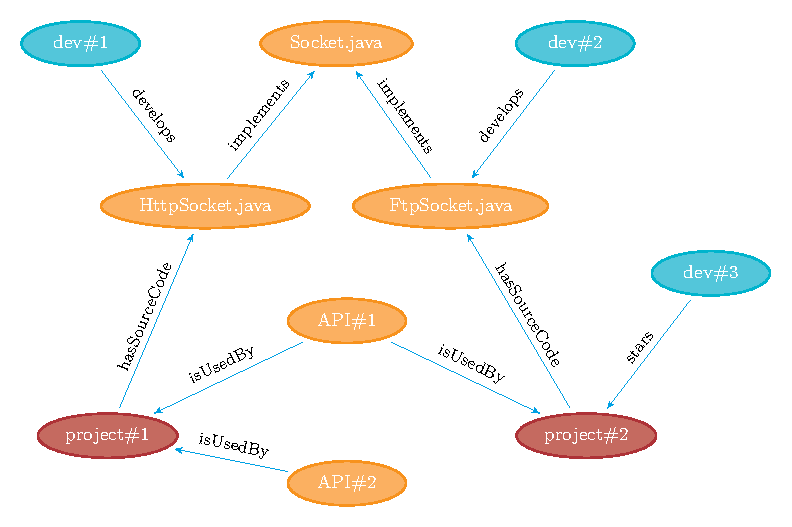
\includegraphics[width=0.60\textwidth]{images/OSSGraph1.pdf}
	\caption{Sample graph-based representation of OSS ecosystems}
	\label{fig:OSSGraph1}
\end{figure}


To demonstrate the utilization of graphs in an OSS ecosystem, we consider an excerpt of the dependencies for two OSS projects, namely \texttt{project\#1} and \texttt{project\#2} in Figure~\ref{fig:OSSGraph1}. Using dependency information extracted from source code and the corresponding metadata (e.g. coming from the tools developed in by Work Package 2), this graph can be properly built to represent the two projects as a whole. In this figure, \texttt{project\#1} contains code file \texttt{HttpSocket.java} and \texttt{project\#2} contains \texttt{FtpSocket.java} with the corresponding edges being marked with the semantic predicate \texttt{hasSourceCode}. Both source code files implement \texttt{interface\#1} being marked by the semantic predicate \texttt{implements}. \texttt{Project\#1} and \texttt{project\#2} are also connected via other semantic paths, such as API \texttt{isUsedBy} highlighted in Figure~\ref{fig:OSSGraph3}. In practice, an OSS graph is much larger with numerous nodes and edges, and the relationship between two projects can be thought as a sub-graph. 

\begin{figure}[h!]
	\centering
	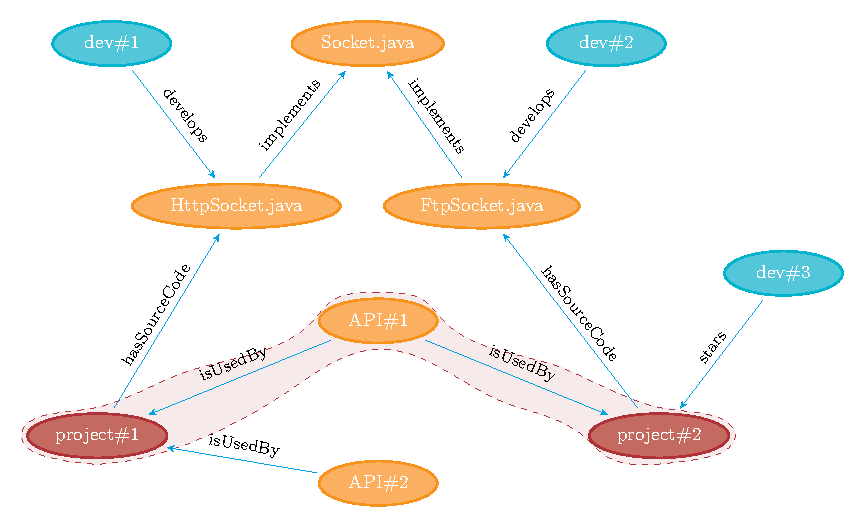
\includegraphics[width=0.60\textwidth]{images/OSSGraph3.pdf}
	\caption{Similarity between OSS projects with respect to API usage}
	\label{fig:OSSGraph3}
\end{figure}



Based on the graph structure, one can exploit nodes, links and the mutual relationships to compute similarity using existing graph similarity algorithms. To the best of our knowledge, there exist several metrics for computing similarity in graph \cite{Blondel:2004:MSG:1035533.1035557},\cite{Nguyen:2015:CRV:2942298.2942305},\cite{Nguyen:2015:ESP:2740908.2742141}. The graph structure also allows for graph kernel methods, which are an effective way to compute similarity \cite{ODMD14a}. Considering Figure~\ref{fig:OSSGraph1}, we can compute the similarity between \texttt{project\#1} and \texttt{project\#2} with regards to the semantic paths between them, e.g. the two-hop path using \texttt{hasSourceCode} and \texttt{implements} (Figure~\ref{fig:OSSGraph2}), or the one-hop path using API \texttt{isUsedBy}. For example, concerning \texttt{isUsedBy}, the two projects are considered to be similar since with the predicate both projects originate from \texttt{API\#1}. The hypothesis is based on the fact that the projects are aiming at creating common functionalities by using common libraries \cite{McMillan:2012:DSS:2337223.2337267},\cite{6671293}.


\begin{figure}[h!]
	\centering
	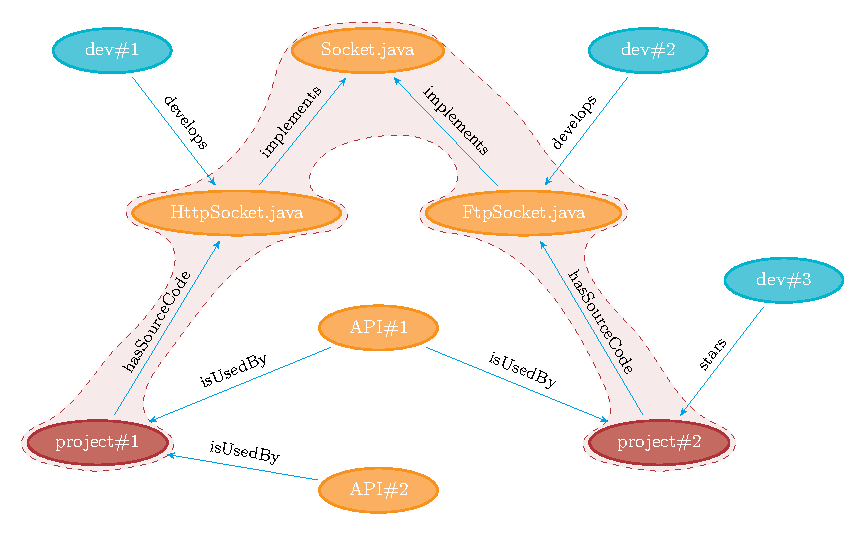
\includegraphics[width=0.60\textwidth]{images/OSSGraph2.pdf}
	\caption{Similarity between OSS projects with respect to source implementation}
	\label{fig:OSSGraph2}
\end{figure}


The representation allows us to compute similarity between other graph components, e.g. developers. Back to Figure~\ref{fig:OSSGraph1}, though there is no direct connection between \texttt{developer\#1} and \texttt{developer\#2}, their similarity can still be inferred from indirect semantic paths, such as \texttt{develops} and \texttt{implements} which are highlighted in Figure \ref{fig:OSSGraph4}.
%
If we consider other semantic paths, we see that the two developers have more in common as they both take part in \texttt{project\#1} and \texttt{projects\#2} represented by \texttt{commits}. To a certain extent, the two developers are considered to be similar, although they are not directly connected. In reality, the connection between \texttt{developer\#1} and \texttt{developer\#2} is enforced by further semantic paths and as a result their similarity can be more precisely computed. The similarities between developers can serve as input for a collaborative filtering recommendation system, with which a developer is recommended a list of projects or libraries that similar developers already worked with \cite{Pazzani2007},\cite{Schafer:2007:CFR:1768197.1768208}. This is an invaluable tool in the context of the CROSSMINER project since it is essential to equip developers with recommendation functionalities to help them increase reusability and productivity.


\begin{figure}[t!]
	\centering
	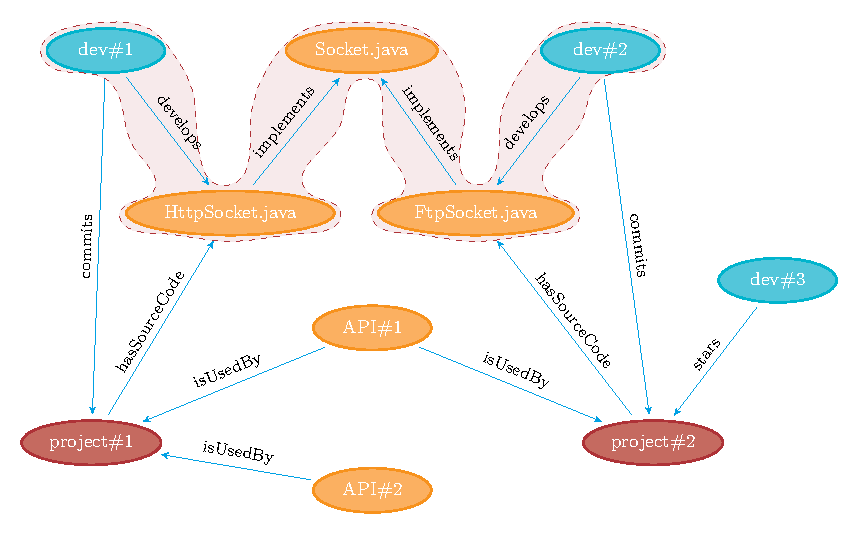
\includegraphics[width=0.60\textwidth]{images/OSSGraph4.pdf}
	\caption{Similarity between developers}
	\label{fig:OSSGraph4}
\end{figure}
\clearpage

%%%%%%%%%%%%%%%%%%%%%%%%%%%%%%%%%%%%%%%%%%%%%%%%%%%%%%%%%%%%%%%%%%%%%%%%%%%% 
\subsection{System Description}
In this section we want to explain our work and what we have done. In order to do this we will use some UML diagram plus a generich high level architecture diagram.
\begin{figure}[H]
	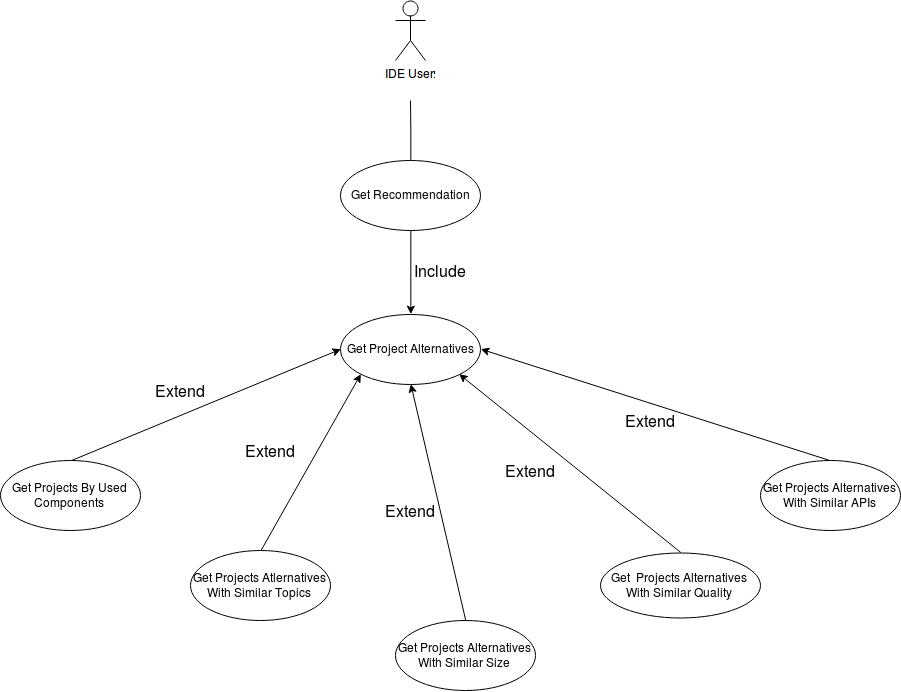
\includegraphics[width=15cm,height=20cm,keepaspectratio]{images/UseCaseDiagram.png}
	\caption{Use Case Diagram}
	\label{fig:UseCase}
\end{figure}
This image, exctracted from CrossSim documentation depicts how a similarity calculator fits inside a real project.
It is clear that in order to provide a meaningful recommendation, it is mandatory to have a similarity calculator better as possible since all the functionality extending the \emph{GetProjectAlternatives} use case, rely on some similarity computation.

\subsubsection{Component Point of View}
\begin{figure}[H]
	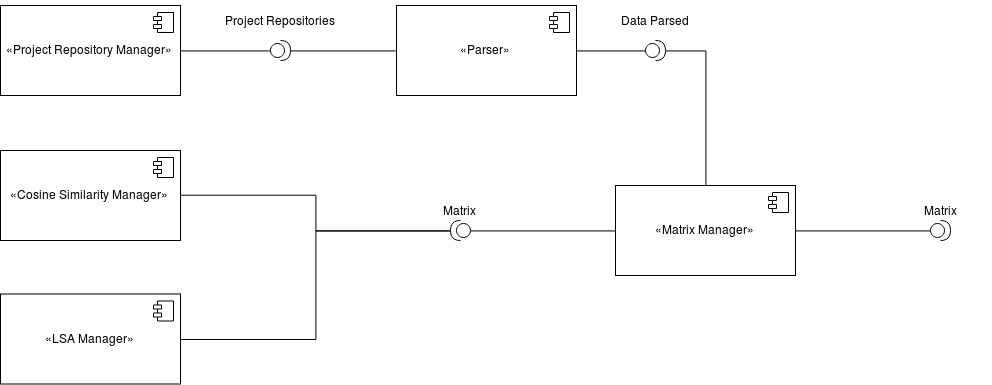
\includegraphics[width=15cm,height=20cm,keepaspectratio]{images/ComponentDiagram.png}
	\caption{Component Diagram}
	\label{fig:Component}
\end{figure}
As you can see there are 5 main components:
\begin{itemize}
	\item Project Repository manager: this is the component who provide the repositories and who manage the file system.
	\item Parser: this component analyzes all the \emph{.java} files in order to retrieve the keywords to create the term-document matrix. As stated before we search for the \emph{JDK} related imports and methods for Clan and any imports, method, variables and field variables for MudaBlue.
	\item Matrix Manager: the matrix manager is the central component, in the sense that manages the creation of the term-document matrix, but not only, it coordinates all the matrices "roaming" during the process. For example the term-document matrix can't be analzed as it is by the SVD component, it requires a rework before.
	\item LSA Manager: here all the operations concerning the Latent Semantic Analsys occurs, from the low-rank matrix reduction to the Singular Value Decomposition.
	\item Cosine Similarity Manager: once the LSA completes his work we can apply the cosine similarity to get the final version of the matrix.
\end{itemize}

\begin{figure}[H]
	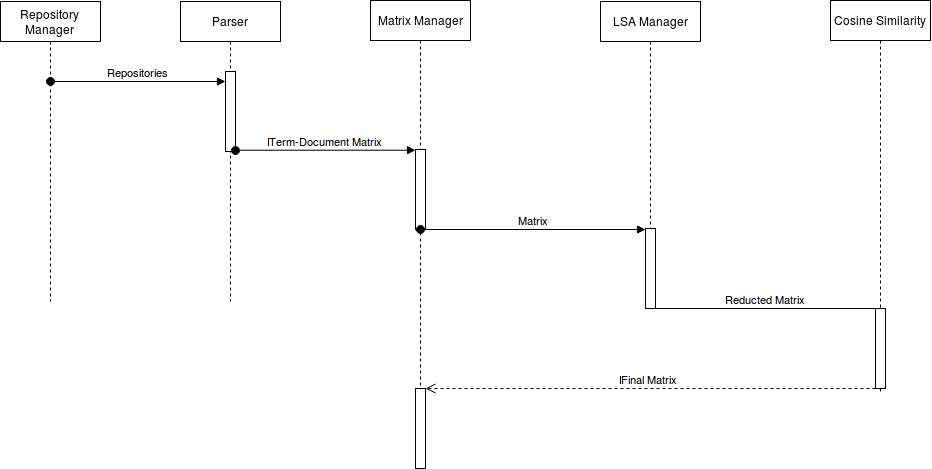
\includegraphics[width=15cm,height=20cm,keepaspectratio]{images/SequenceDiagram.png}
	\caption{Sequence Diagram}
	\label{fig:Sequence}
\end{figure}

In the figure \ref{fig:Sequence} we can see the sequence diagram.
When the process starts, the repository manager analyzes the file system in order to provide all the repositories to be analyzed. It also check if the parsing has been occurred before to such repositories, this is due the extremely high consumption of memory, so we splitted the phases in two moments.\\
When we know what are the repositories to be analyzed we can start, as explained before for MudaBlue and Clan the terms are different, but we still use the same library in both cases \emph{Java Parser}.\\
The outcome will be a term-document matrix worked by the Latent Semantic Analysis manager.
First of all we invoke the \emph{commons math} for decomposing the matrix, then we can multiply them back in order the get the LSA matrix.\\
At this stage we just need to take the matrix and then apply the cosine similarity, for each vector of the matrix we calculate the cosine with all the others vectors. In this way we will get a final matrix of \emph{580 x 580}.
The final matrix can be taken for further analysis or anything that we need.

\clearpage

\subsubsection{Description}
\begin{figure}[H]
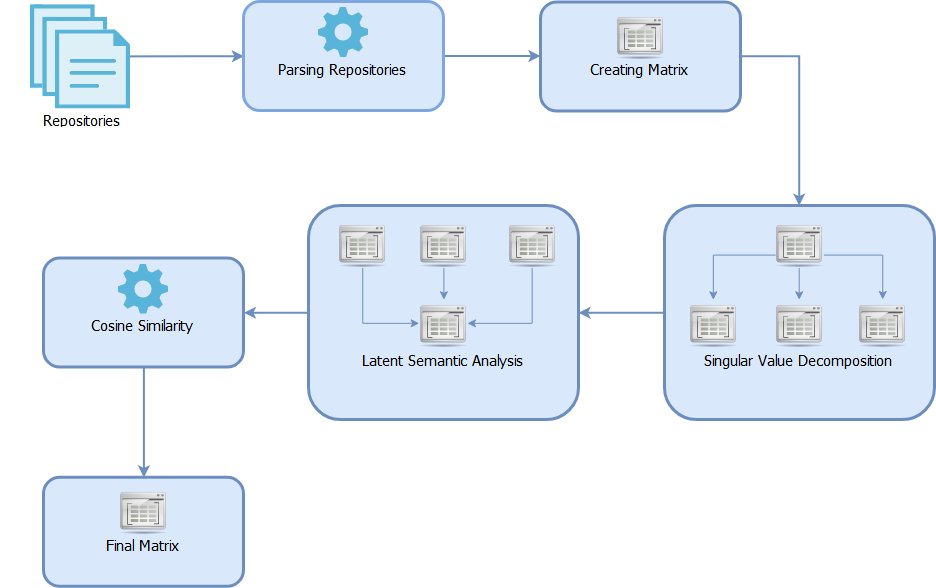
\includegraphics[width=15cm,height=20cm,keepaspectratio]{images/Architecture.png}
\caption{System Structure}
\end{figure}

In this image is depicted the general architecture of the implemented systems, as you can see the systems share the same architecture with some differences that will be discussed later.
As you can see, the process consist of 7 steps.
\begin{itemize}
 \item Retrieving the dataset, in this case a folder with all 580 repositories.
 \item All these repositories are analyzed, and any \emph{.java} file is parsed.
 \item For each repository a vector that contains all the frequencies for each term found is created, and then added in a matrix. 
 \item The SVD procedure, decomposing the matrix in other 3.
 \item The matrices are multiplied back to realize the LSA procedure.
 \item For each vector, we count the cosine similarity with all the others.
 \item Now we have the final matrix, where any repositories is compared to all the others.
\end{itemize} 

\subsubsection{System Details}

\begin{figure}[H]
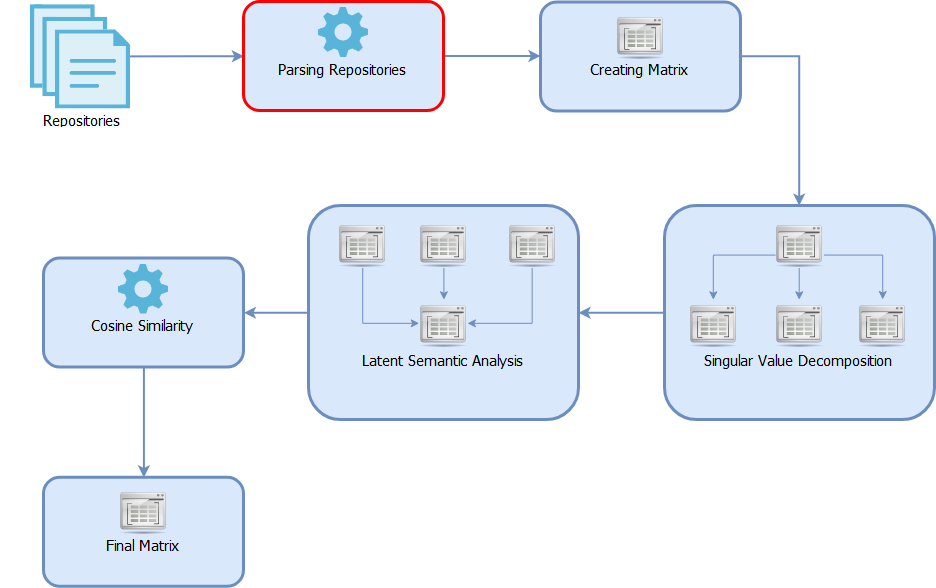
\includegraphics[width=15cm,height=20cm,keepaspectratio]{images/Architecture1.png}
\caption{Parsing}
\end{figure}

Parsing: The first step is clearly parsing the java files of the 580 repositories. We used the javaparser library to directly access
the main components of the files (import and method invocation for CLAN, import, method declaration, variables and field variables for MudaBlue). For each repository we created a relative .txt file containing the frequencies, for the CLAN approach such terms are filtered by searching only the terms belonging to the Java JDK. All these terms are merged in another file, called mainlist.txt which is used to avoid reps. The idea is parsing the files and compare with the mainlist.txt to add new terms, and then count, for each terms how many times appears inside the files. So the result will be a vector of numbers.

\begin{figure}[H]
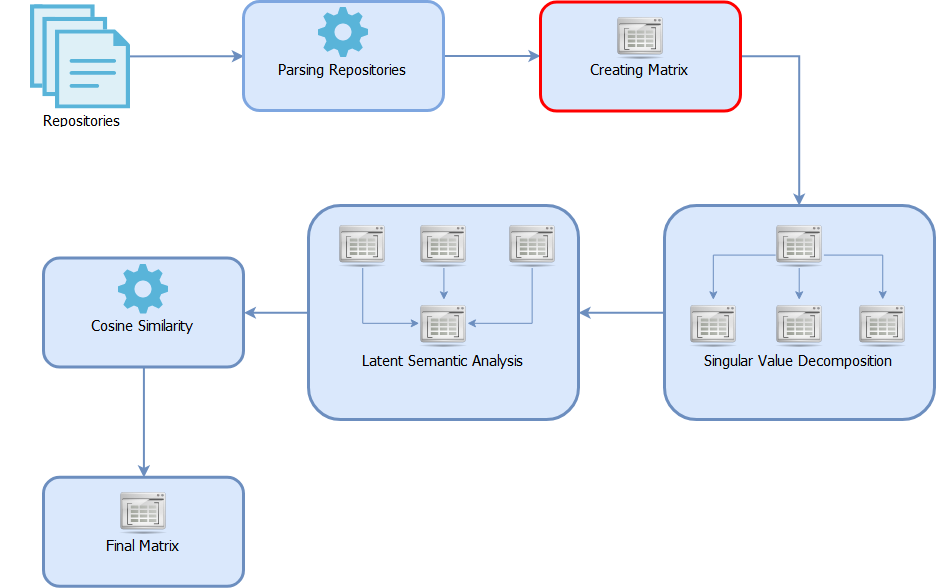
\includegraphics[width=15cm,height=20cm,keepaspectratio]{images/Architecture2.png}
\caption{Matrix Creation}
\end{figure}

Matrix Creation: Once all the repositories are analyzed we can procede in creating the term-document matrix. The matrix is created using the library \emph{apache commons math3} and in particular these components:
\begin{itemize}
\item ArrayRealVector.
\item RealMatrix.
\item RealVector.
\end{itemize}
Each files contains only his own terms naturally, so the idea is, once the parsing process is done, to count how many terms we have and then, adding many zeros as many terms are missing. To clarify, imagine that we have 3 documents \emph{A,B,C} for 10 different terms.
Now if we examine the document A, we might discover 4 terms, this means that the other 6 terms are missing here, so can be marked as 0. 
For the document B, we might find out 2 new terms, and so on.

\begin{figure}[H]
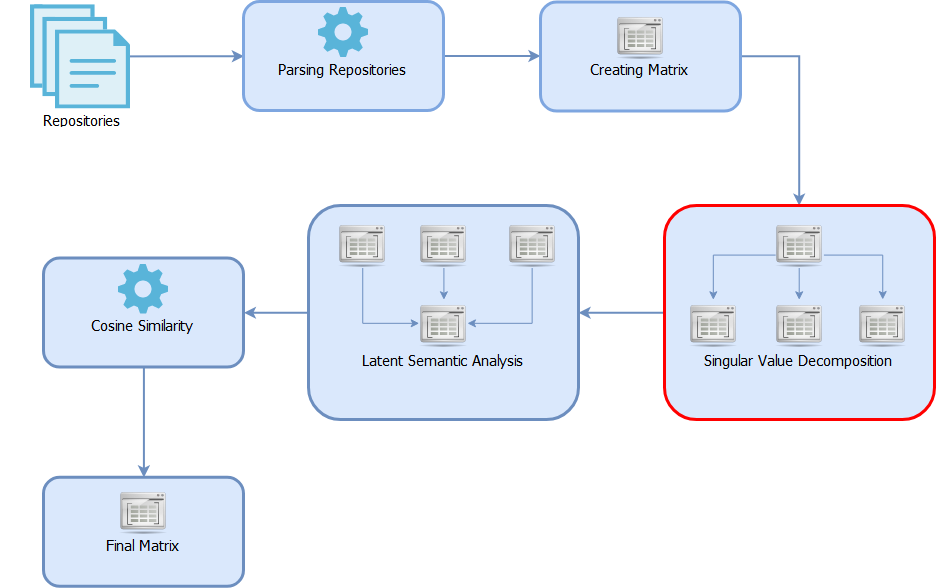
\includegraphics[width=15cm,height=20cm,keepaspectratio]{images/Architecture3.png}
\caption{Singular Value Decomposition}
\end{figure}

SVD: As stated before the svd operation consist in decomposing the main matrix in other 3.

\begin{equation}
A_{mn}=U_{mm}S_{mn}V_{mn}^{T}
\end{equation}

in which

\begin{itemize}
	\item $U_{mm}$: Orthogonal matrix.
	\item $S_{mn}$: Diagonal matrix.
	\item $V_{mn}^{T}$: The transpose of an orthogonal matrix.
	\item $X$: Low Rank matrix.
\end{itemize}

Such operation are provided by \emph{math3 linear SingularValueDecomposition}.
So we invoke the methods passing as parameter the term-document matrix.
As you can see this operation was already available in the library, so we just retrieved the results of the operation.

\begin{figure}[H]
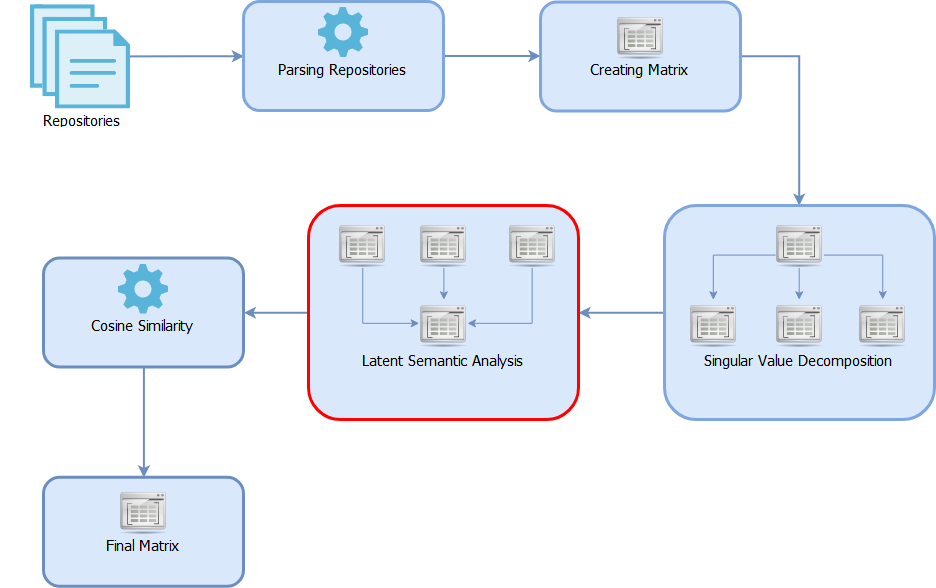
\includegraphics[width=15cm,height=20cm,keepaspectratio]{images/Architecture4.png}
\caption{Latent Semantic Analysis}
\end{figure}

LSA: Unfortunately an implementation of Latent Semantic Analysis wasn't available, so we re-implemented from scratch.
Basically we multiplied the 3 matrix provided by the \emph{SVD} procedure, the important point is the value \emph{k} for the reduced rank, we selected a value of total $\frac{repository}{2}$. As explained in the Dumais paper, this value should be selected empirically. 
Here we got a very big issue since the
$Memory\,in\,gigabytes\,=\,\frac{(columns*rows*8)}{(1024*1024*1024)}$ is required for a matrix, for MudaBlue we got an amount of 700000 distinct terms for a total of 3GB of dedicated memory just for matrix, without cosidering any kind of operation. This is due to the fact that MudaBlue considers many different terms from a file. Clan instead, focusing only on the the import and method that belongs to the \emph{JDK}, reduced greatly the number of distinct terms. The main solution was to increase the available memory for eclipse up to 8GB. Even though this memory space, we got many crashes, so we spent some time in refactoring the code to save memory, e.g. deleting unused data structure, using more light structures and so on.

\begin{figure}[H]
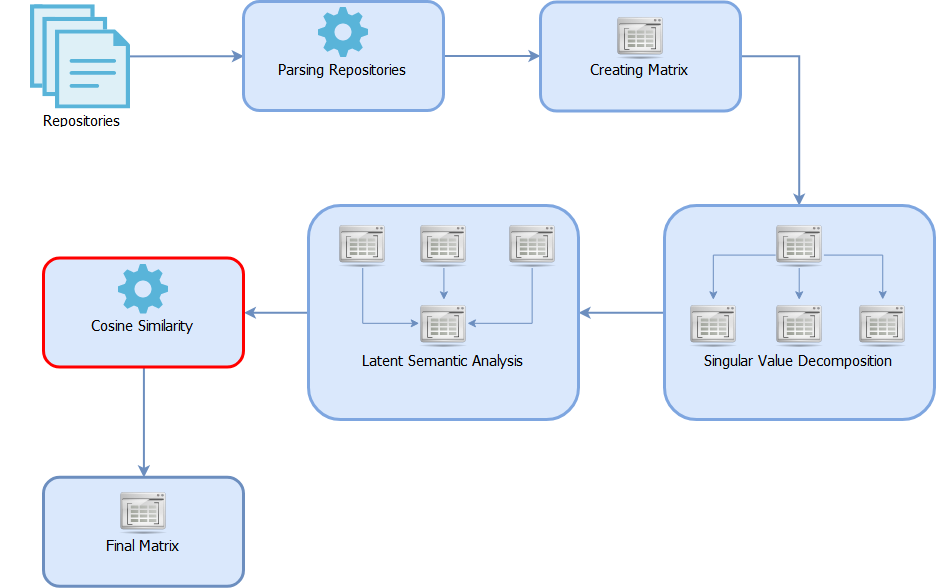
\includegraphics[width=15cm,height=20cm,keepaspectratio]{images/Architecture5.png}
\caption{Cosine Smilarity}
\end{figure}

As stated before, by cosine similarity we mean a measure of similarity between two non-zero vectors of an inner product space that measures the cosine of the angle between them, that is, how much they are close or far each other. As for the \emph{LSA} we re-implemented the operation from scratch, so the method take as input two vectors and computes the operation, such vectors are taken from the \emph{LSA} matrix, in such a way that every couple is taken into account. Since in the final matrix we will have the simlarity between \emph{repo1 - repo2} and \emph{repo2 - repo1}, we computed the cosine only in the upper triangular matrix to cut half of the calculation.

\begin{figure}[H]
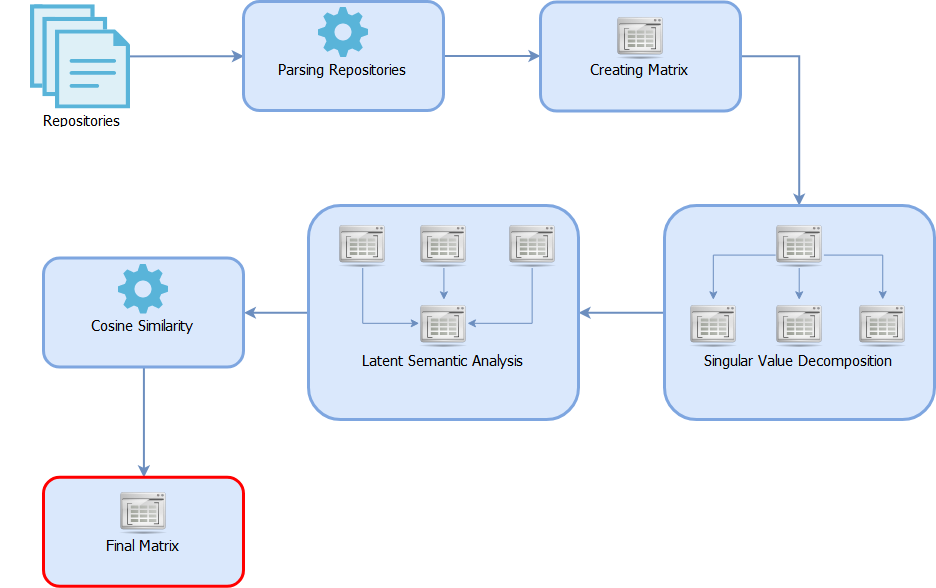
\includegraphics[width=15cm,height=20cm,keepaspectratio]{images/Architecture6.png}
\caption{Final Matrix}
\end{figure}

At this stage the matrix is complete with \emph{580 * 580} in dimension, and with values between \emph{0.0} and \emph{1.0}.
This matrix is actually a collection of vectors, representing the similarity of a project with all the other projects.
To be more formal the final matrix $\| M \|$ is square matrix whose rows and columun represents projects. In particular, for any two project $P_i$ and $P_j$, each element of the matrix $M_{i,j}$ represents the similarity score defined as follows: \\

\begin{equation}
  M_{i,j}=\begin{cases}
    0\leq M \leq 1 \; \; \; \text{if i} \neq \text{j}\\
    \\
    1 \; \; \; \text{if i = j}.
  \end{cases}
\end{equation}\\

There is one more step for CLAN, since the approach consider the matrices separately, that is, at this stage we have two different matrices, one for the imports and one for the methods. So we have to sum up both in order to get the final one.

%%%%%%%%%%%%%%%%%%%%%%%%%%%%%%%%%%%%%%%%%%%%%%%%%%%%%%%%%%%%%%%%%%%%%%%%%%%%%%%%%%%%%%%%%%%
\newpage
\subsection{Tools and Libreries}
During the experience, the work has been done using Eclipse IDE Oxygen .2, and using the following libreries.
\begin{itemize}
\item org.eclipse.jdt.core 3.10.0. 
This is the core part of Eclipse's Java development tools. It contains the non-UI support for compiling and working with Java code, including the following:
	\begin{itemize}
	\item an incremental or batch Java compiler that can run standalone or as part of the Eclipse IDE
	\item Java source and class file indexer and search infrastructure
	\item a Java source code formatter
	\item APIs for code assist, access to the AST and structured manipulation of Java source.
	\end{itemize}
\item eclipse-astparser 8.1. This is used to analyze the AST at runtime on Eclipse.
\item commons-math3 3.6.1 Commons Math is a library of lightweight, self-contained mathematics and statistics components addressing the most common problems not available in the Java programming language or Commons Lang. 
In particular used to compute the SVD, singular value decomposition.
\item commons-text 1.2. Apache Commons Text is a library focused on algorithms working on strings. 
\item javaparser-core 3.5.14. This is a library for parsing the java files.
\item ejml 0.33. Efficient Java Matrix Library (EJML) is a linear algebra library for manipulating real/complex/dense/sparse matrices. Its design goals are; 1) to be as computationally and memory efficient as possible for both small and large matrices, and 2) to be accessible to both novices and experts.These goals are accomplished by dynamically selecting the best algorithms to use at runtime, clean API, and multiple interfaces.
\end{itemize}

%%%%%%%%%%%%%%%%%%%%%%%%%%%%%%%%%%%%%%%%%%%%%%%%%%%%%%%%%%  